\chapter{Laserfysik}
Ordet laser er en forkortelse for \emph{Light Amplification by Stimulated Emission of Radiation}, som på dansk vil oversættes til \emph{lysforstærkning ved stimuleret emission af stråling}. Laseren har en stor betydning såvel for fysikere som for den almindelige borger, da laserteknologien bl.a. bruges i stregkodescannere,
laserprintere, fiberoptik og som en del af medicinske og kosmetologiske behandlinger. I fysikkens verden bruges lasere til bl.a. at studere kvantemekaniske systemer eksperimentelt eller til at observere fjerne astronomiske objekter med kæmpe store teleskoper. 


\section{Atomet}
I forkortelsen for laser indgår ordet \emph{lysforstærkning}. For at lave en laser skal vi altså forstærke noget lys. Dette lys kommer ud fra vekselvirkinger mellem fotoner og elektroner, hvoraf sidstnævnte sidder i et atom. Atomet består af en kerne af protoner og neutroner, og elektronskaller/elektronskyer, hvor elektronerne befinder sig. Fotoner kaldes også lyspartikler eller lyskvanter og siges at bære på lyset. 

En kvant kan defineres som den mindste udelelige del af et stof. Forestil dig et stykke kridt, der bliver hakket så meget i stykker, at du til sidst har et stykke, som du ikke længere kan hakke over. Dette stykke vil defineres som en kvant. Elementer på denne størrelse er meget, meget små og befinder sig på en skala hvor en beskrivelse af fysikken kræver \emph{kvantemekanik}. På den kvantemekaniske skala gælder princippet om \emph{partikel-bølge-dualitet}, der siger, at alle kvanter besidder både partikelegenskaber og bølgeegenskaber. En foton er altså ikke kun en partikel eller ikke kun en bølge, men besidder altså egenskaber fra begge fænomener. På trods af det, tegnes en foton altid som en bølge.  

En foton har energien 
\begin{equation}
E_{\text{foton}} = h\nu = \frac{hc}{\lambda},
\end{equation}
hvor $\nu$ er frekvensen af lyset, $c$ er lysets hastighed i vakuum, $h$ er Plancks konstant og $\lambda$ er bølgelængden af lyset. Bemærk her, at $\nu$ og $\lambda$ er bølgeegenskaber. 

Fotoner eller lys er ikke blot bølger, men faktisk \emph{elektromagnetiske bølger}. Vi vil ikke gå i dybden med dem i dette kapitel, men de bliver studeret nærmere i valgfaget af samme navn. 
Kort beskrevet består en elektromagnetisk bølge af et elektrisk felt og et magnetfelt, der altid står vinkelret på hinanden. Felterne kan samtidigt beskrives som bølger, der står og svinger. For nu, er det nok at huske, at lys eller fotoner består af et elektrisk felt og et magnetfelt. 

Fotonens partikelegenskaber kommer til udtryk ved, at den kan vekselvirke med bl.a. en elektron ved enten at blive absorberet (afgive energi) eller at blive emitteret (udsende energi). Fotonen og elektronen kan vekselvirke på flere måder, og de tre vigtigste for dette emne er \emph{stimuleret absorption}, \emph{spontan emission} og \emph{stimuleret emission}.

Elektronerne befinder sig som sagt i elektronskallerne i et atom. Skallerne betegnes ofte som energitilstande, hvor i elektronerne befinder sig. Den laveste energitilstand findes tættest på kernen og kaldes for \emph{grundtilstanden}, hvor de øvrige tilstande med højere energier kaldes \emph{exciterede tilstande}. Man siger, at atomet har diskrete energitilstande, da en elektron ikke kan befinde sig mellem to forskellige energitilstande. Vi antager for simpelhedens skyld, at vi har at gøre med et 2--niveau system, som består af grundtilstanden og én exciteret tilstand. 


\subsection{Stimuleret Absorption}
Befinder en elektron sig i grundtilstanden med energi $E_1$ i det nævnte 2--niveau system, kan den exciteres til den exciterede tilstand med energi $E_2$ ved at absorbere en indkommende foton, der afgiver alt sin energi til elektronen. Fotonens energi skal svare til energiforskellen mellem tilstandene, da det vil være den energi, det kræver at flytte en elektron fra grundtilstanden til den exciterede tilstand, altså skal energien af fotonen være
\begin{equation}
E_{\text{foton}} = h\nu =  E_2-E_1.
\label{eq:efot}
\end{equation}


Processen kaldes stimuleret absorption (se Figur \ref{fig:vekselvirkning}a). Den er stimuleret fordi atomet må påvirkes af lys før denne proces sker. Processen sker altså ikke spontant. 

\subsection{Spontan Emission}
Når en elektron har absorberet en foton vil den som sagt exciteres til en exciteret tilstand. Den exciterede tilstand vil være ustabil og elektronen vil før eller siden falde tilbage til grundtilstanden. Den bevæger sig altså nu fra en tilstand med en højere energi til en tilstand med en lavere energi (se Figur \ref{fig:vekselvirkning}b). Da energien skal være bevaret, vil der være noget energi tilovers. Denne energi vil udsendes i form af en foton, som vil have den samme energi, det kræver at excitere elektronen fra grundtilstanden til den exciterede tilstand, altså ligning \ref{eq:efot}. 

Processen kaldes for spontan emission, og kræver ikke nogen påvirkning, hvorfor processen er spontan. 

\subsection{Stimuleret Emission}
Hvis en elektron i den exciterede tilstand ikke henfalder spontant ved spontan emission, kan den vekselvirke med en foton og derefter falde tilbage til grundtilstanden (se Figur \ref{fig:vekselvirkning}c). Da energien stadig skal være bevaret må der udsendes to fotoner med samme energi givet ved ligning \ref{eq:efot}. 

Denne proces kaldes stimuleret emission, fordi elektronen påvirkes af udefrakommende lys, og derfor ikke er spontan. 

Stimuleret emission er det fysiske fænomen, der udnyttes i en laser, i det det er muligt at genere mere lys ved at påvirke atomer med fotoner(lys). Da energien af fotonerne afhænger af bølgelængden, vil bølgelængden af de to udsendte fotoner også være den samme. 

\begin{figure}[h!]
  \centering
  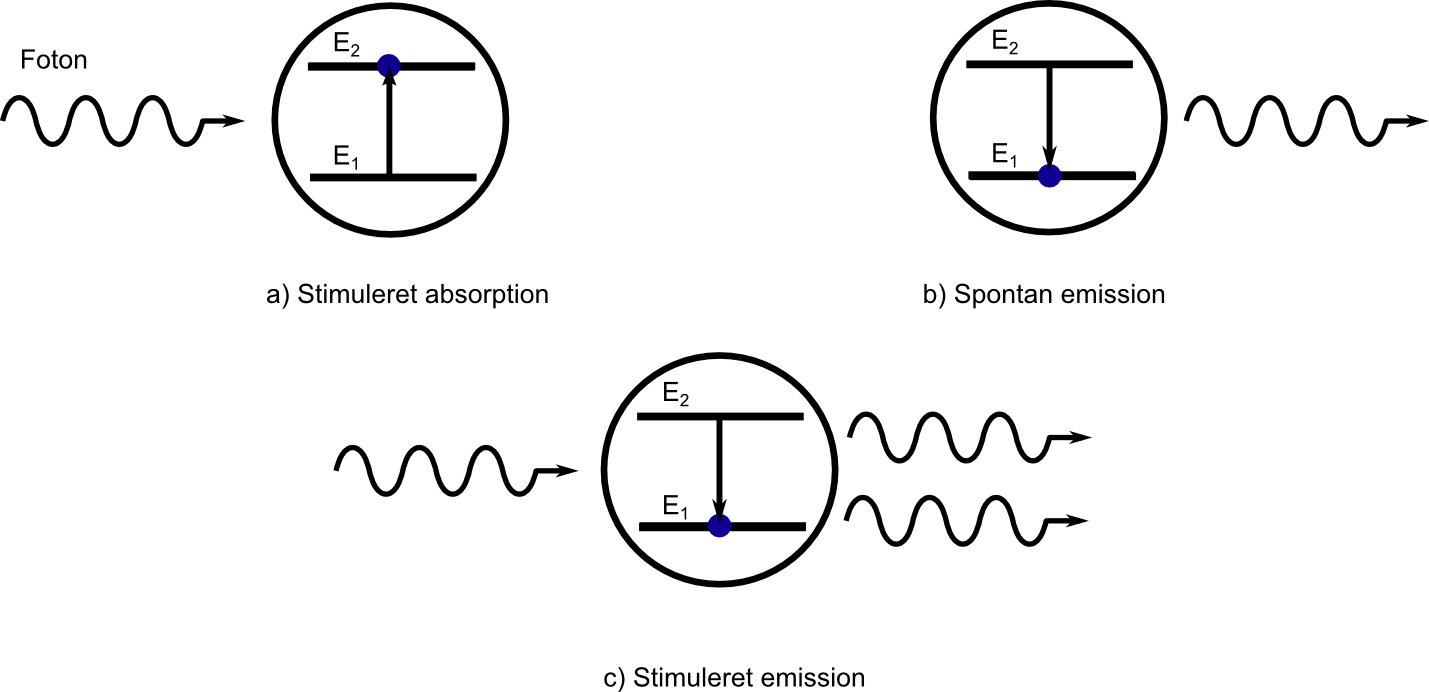
\includegraphics[width=0.8\textwidth]{Laserfysik/vekselvirkning2.png}
  \caption{2-niveau atom bestående af grundtilstand med energi $E_1$ og exciteret tilstand med energi $E_2$. a) Stimuleret absorption: elektron absorberer en foton og springer til den exciterede tilstand. b) Elektron henfalder ved spontan emission til grundtilstanden og udsender en foton. c) Elektron i den exciterede tilstand absorberer en foton og henfalder til grundtilstanden ved udsendelse af to fotoner med samme energi. }
  \label{fig:vekselvirkning}
\end{figure}

\section{Et Laser System}
Vi antager stadig at have et 2--niveau system. Flere--niveau systemer beskrives senere. Fremover vil vi se på flere atomer end blot ét, hvorfor vi beskriver et exciteret atom, som et atom, hvori en eller flere elektroner har absorberet en foton og er sprunget til en exciteret energitilstand.   

For at genere laserlys ved vi nu, at vi skal påvirke elektroner i exciterede tilstande med lys for at lave stimuleret emission. Hvis denne laser skal blive ved med at lyse må processen nødvendigvis skulle gentages igen og igen. 

Et laser system består af flere elementer, der tilsammen hele tiden sørger for at forstærke lyset og sende en lille del af det ud. Dette afsnit beskriver disse elementer, som også ses på Figur \ref{fig:lasersystem}. 

\begin{figure}[h!]
  \centering
  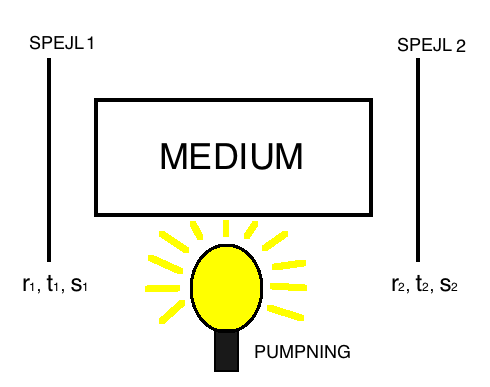
\includegraphics[width=0.6\textwidth]{Laserfysik/lasersystem.png}
  \caption{Lasersystemet består af et medium, en optisk laser kavitet bestående af to spejle og en pumpe, der her illustreres som en lampe. Mediet skal være et forstærkende medium for at opnå population inversion, og $r_1>r_2$ såfremt man ønsker et laser output gennem spejl 2.}
  \label{fig:lasersystem}
\end{figure}

\subsection{Medium}
Det første element er et \emph{medium}, der skal forstærke lys ved stimuleret emission. Mediet kan både være på fast, flydende eller gas form. Uanset hvilken form mediet er på, er stimuleret emission det fysiske fænomen, der udnyttes for at genere lys. Det kan dog være forskelligt, hvordan en elektron går fra én energitilstand til en anden. En diode laser har f.eks. et medium på fast form. Faste stoffer har energibånd i stedet for diskrete energitilstande, hvorfor energiovergange beskrives på en anden måde. 

Mediet kan enten være et \emph{forstærkende/gevinst} medium eller et \emph{absorberende} medium. 
Vi skriver densiten af atomer i grundtilstanden som $N_1$ og densitet af atomer i den exciterede tilstand som $N_2$. Det specifikke antal af atomer beskrives senere. Hvis $N_1>N_2$ vil mediet absorbere mere end forstærke, fordi der er flere atomer i grundtilstanden til at absorbere noget indkommende lys, end der er atomer i den exciterede tilstand til at henfalde til grundtilstanden og udsende lys ved enten stimuleret eller spontan emission. Mediet vil da kaldes et absorberende medium. Hvis $N_2>N_1$ vil mediet forstærke mere lys end det vil absorbere, og mediet kaldes da et forstærkende eller gevinst medium (eng: gain medium). 

$N_2-N_1$ kaldes \emph{population inversion} og er et vigtigt begreb indenfor laserfysik. Et forstærkende medium kræver altså en positiv population inversion for at kunne forstærke lys. Er population inversion derimod negativ er mediet absorberende. 

\subsection{Optisk Laser Kavitet}
Mediet placeres mellem to spejle, der udgør en \emph{optisk laser kavitet}, og som også kaldes en \emph{resonator} i nogle sammenhænge. Spejlene sørger for at reflektere lyset, der generes i mediet, tilbage i mediet, så processen for stimuleret emission gentages. Derudover har det ene spejl en mindre reflektivitet end det andet, således at dette spejl også transmitterer noget af lyset, hvilket er det lys, vi ser som laserlyset. 

Spejlene besidder tre koefficienter, $r, t$ og $s$, hvor $r$ er refleksionskoefficenten, $t$ er transimisionskoeficienten og $s$ er spredningskoefficienten. De har alle en værdi mellem 0 og 1, hvor $r=1$ svarer til at spejlet er 100\% reflekterende. Det vil dog kræve, at spejlet hverken transmitterer eller spreder noget af lyset, i det der gælder at 
\begin{equation}
r + s + t = 1.
\end{equation}

Bemærk altså, at der også går noget lys tabt ved spejlene i form af spredning, og dette beskrives ved $s$. 

Da lys(fotoner) har bølgeegenskaber, kan der opstå en stående bølge mellem de to spejle. Dette er ækvivalent til en stående bølge på en snor, hvor begge ender af snoren er fastgjort, hvorefter snoren sættes i svingninger. Bølgens svingninger \emph{interferer} med hinanden, så der opstår destruktiv og konstruktiv inteferens. Destruktiv inteferens opstår, når to svingningerne eller bølger udslukker hinanden, og ses altså som et knudepunkt på snoren, hvor konstruktiv inteferens forstærker to svingninger eller bølger og danner en bølge-- top eller dal. 

Lyset vil på samme måde intefere inde i den optiske kavitet, men vil kun danne stående bølger, hvis afstanden mellem spejlene $L$ opfylder 
\begin{equation}
L = n\frac{\lambda}{2}, \,\,\,\,\,\, n =1,2,3...,
\end{equation}
hvor $n$ er et heltal og $\lambda$ er bølgelængden af lyset. Stående bølger af lys kan altså opstå, hvis længden af kaviteten er et helt antal halve bølgelængder. Når en stående bølge dannes siges lyset at svinge ved \emph{resonans}, lyset har således også en \emph{resonansfrekvens}. 

Figur \ref{fig:bolger} viser stående bølger i en kavitet ved variende længder. 

\begin{figure}[h!]
  \centering
  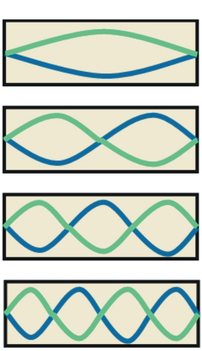
\includegraphics[width=0.35\textwidth]{Laserfysik/standing_waves_only.png}
  \caption{Stående bølger i en kavitet, hvis længde varierer mellem (øverst til nederst) $L = \frac{\lambda}{2}, \,\, L = \lambda, \,\, L = \frac{3\lambda}{2}...$}
  \label{fig:bolger}
\end{figure}

For at kunne forstærke lys i en optisk kavitet, er det derfor vigtigt, at justere længden af kaviteten, så stående bølger kan opstå for den ønskede bølgelængde.  
% spørgsmål til dem om dette. Kan de gennemskue hvorfor?

\subsection{Pumpe}
Det sidste element er en pumpe. Pumpen har til formål at sørge for at flest mulige atomer befinder sig i en exciteret tilstand, så de kan udsende lys ved stimuleret emission. Pumpen kan f.eks. være en lampe, der udsender fotoner med den rette energi, således at elektronerne i atomerne absorberer fotonerne ved stimuleret absoprtion. Processen kaldes \emph{pumpning}. 

\section{Absorption/Gevinst Koefficient og Intensitet}
Vi ønsker at beskrive ændringen i intensitet\footnote{Intensitet er et mål for styrken af et fænomen. I fysik defineres intensitet som energi pr. tid pr. areal, altså $I = \frac{E/t}{A}$} af lyset, der bevæger sig inde i mediet. Med denne beskrivelse kan vi senere bestemme en tærskelværdi for, hvornår lasing kan opnåes. Til beskrivelsen af intensiteten hører også en \emph{absorption/gevinst koefficient}, som beskriver ændringen i intensiteten af det propagerende lys gennem mediet i forhold til stimuleret emission og absorption. 

Vi husker, at lys består af et elektrisk felt og et magnetfelt. Intensiteten af lyset gennem mediet er 
\begin{equation}
I = uc,
\label{eq:intensitet}
\end{equation}
hvor $c$ er lysets hastighed i vakuum og $u$ er \emph{feltenergi densiteten}, der afhænger af lysets elektriske felt og magnetfelt. Energi densitet beskriver altså mængden af energi, der ligger (eller er lagret) i det elektriske felt og magnetfelt, vi kan kalde denne energi for den \emph{elektromagnetiske energi}. 

Vi ønsker nu at bestemme med hvilken rate den elektromagnetiske energi forlader et volumen, der udgør mediet. Volumen er givet som areal $\times$ længde, hvor arealet angives som $A$. Forestil dig en kasse, der udgør mediet (se Figur \ref{fig:intenmed}). Kassens ender har et areal på $A$ og længden af kassen går fra punktet 0 til punktet $Z$, således at kassen har længden $Z$. Et punkt mellem 0 og $Z$ betegnes $z$. I punktet $z$ er raten hvormed elektromagnetisk energi passerer $I(z)A$, hvor $I(z)$ er intensiteten af lyset i punktet $z$. I et andet punkt $z+\Delta z$ er raten hvormed elektromagnetisk energi passerer $I(z+\Delta z)A$. 

\begin{figure}[h!]
  \centering
  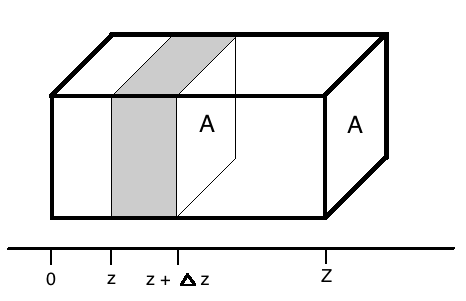
\includegraphics[width=0.5\textwidth]{Laserfysik/intensitetmedium.png}
  \caption{Medium illustreret med en kasse med længde $Z$. Vi ønsker at bestemme hvor intensisten, der forlader det grå volumen givet ved $A\Delta z$. $\Delta z$ kan vælges frit, og kan derfor også betegne hele længdens kasse. Dette er blot en skitse.}
  \label{fig:intenmed}
\end{figure}

Vi ønsker at bestemme differencen mellem, hvor meget energi der passerer igennem de to punkter $z$ og $z+\Delta z$, idet, det vil give raten hvormed den elektromagnetiske energi falder i volumet $A\Delta z$. Differencen er 

\begin{equation}
\left[I(z+\Delta z)-I(z)\right]A \approx \left[ I(z) + \d{I}{z}\Delta z - I(z) \right]A = \d{}{z}(IA)\Delta z
\label{eq:rate}
\end{equation}

når det antages, at $\Delta z$ er meget lille. Raten hvormed elektromagnetisk energi forlader et volumen må være lig med ændringen i elektromagnetisk energi pr. tid i det samme volumen. Den elektromagnetiske energi er energi densitet $\times$ volumen, og man får da at 

\begin{equation}
\d{}{t}(uA\Delta z) = -\d{}{z}(IA)\Delta z. 
\label{eq:rate2}
\end{equation}

Da ligning \ref{eq:rate} beskriver den elektromagnetiske energi, der \emph{forlader} volumet, må ændringen i energien nødvendigvis være negativ. Hverken $A$ eller $\Delta z$ ændrer sig og er derfor konstante. Fra ligning \ref{eq:intensitet} fås $u=\frac{I}{c}$, og ligning \ref{eq:rate2} kan da skrives på formen

\begin{equation}
\frac{1}{c}\d{I}{t} + \d{I}{z} = 0.
\label{eq:kontinuitet}
\end{equation} 

Ligning \ref{eq:kontinuitet} kaldes for \emph{kontinuitetsligningen} og beskriver, hvordan intensiteten opfører sig i tid og rum. 

Vi har indtil nu antaget, at kassen vist i Figur \ref{fig:intenmed} er tom, dvs. lyset bevæger sig i vakuum. I et lasersystem er mediet ikke tomt, men fyldt med et materiale, der kan forstærke lys ved stimuleret emission. Højresiden i ligning \ref{eq:kontinuitet} skal derfor ikke være 0, men skal beskrive raten pr. volumen hvormed den elektromagnetiske energi ændrer sig i forhold til mediet, dvs. i forhold til absorption og stimuleret emission. Raten er proportional til \emph{absorption koefficienten} eller \emph{gevinst koefficienten}, der skrives som hhv. $g(\nu)$ og $a(\nu)$, og afhænger altså af frekevensen af lyset. Vi vil ikke gennemgå en detaljeret beregning af disse men blot give udtrykket 

\begin{equation}
g(\nu) = \sigma(\nu)(N_2-N_1) = -a(\nu). 
\label{eq:gevinst}
\end{equation}

Er mediet et forstærkende, dvs. $N_2>N_1$ benyttes $g(\nu)$, mens et absorberende medium benytter den positive absoprtionskoeffcient 

\begin{equation}
a(\nu) = \sigma(\nu)(N_1-N_2) = -g(\nu). 
\end{equation}

$\sigma(\nu)$ er \emph{tværsnittet} og beskriver en sandsynlighed for, hvor mange atomer, der induceres til at undergå stimuleret emission eller absorption. Tænker man på tværsnittet som et areal, kan man forklare det ved, at enhver foton, som befinder sig inden for dette areal, vil inducere et atom til at undergå stimuleret emission eller absorption. 

Ligning \ref{eq:kontinuitet} bliver så 
\begin{equation}
\left(\frac{1}{c} \d{}{t} + \d{}{z}\right)I = \sigma(\nu)\left(N_2-N_1\right)I = g(\nu)I
\label{eq:konti2}
\end{equation}

Ligning \ref{eq:konti2} beskriver ændringen i intensiteten i både rum og tid, men oftest kan man antage, at intensiteten ikke ændrer sig i tid (dvs. $\d{I}{t} = 0$), og man får da, det der hedder en \emph{stationær ligning}. Den stationære ligning for ændringen i intensitet er så 

\begin{equation}
\d{I}{z} = g(\nu)I. 
\label{I_diff}
\end{equation}

Løsningen til denne differentialligning er 
\begin{equation}
I(z) = I(0)e^{g(\nu)z}. 
\label{I_losning}
\end{equation}

Intensiteten af lyset, der udbreder sig gennem mediet vokser altså eksponentielt med afstanden $z$ såfremt mediet er forstærkende. Er mediet istedet absorberende, vil intensiteten aftage eksponentielt gennem mediet. 


\section{Tærskelværdi}
Som tidligere beskrevet, er mediet placeret mellem to spejle, der udgør en optisk laser kavitet. I kaviteten må lyset nødvendigvis hele tiden forstærkes for at opretholde lasing, det kræver at forstærkningen konstant må overgå de tab, der måtte være i lasersystemet. Tabene kan f.eks. komme fra spredning og absorption i spejlene. Det betyder, at der er en nedre grænse på gevinst koefficienten givet ved ligning \ref{eq:gevinst}, hvor lasing under denne ikke kan forekomme. Værdien, som $g(\nu)$ skal være større end eller lig med kaldes for tærskelværdien (eng: threshold). 
Vi bestemmer tærskelværdien ved at vurdere intensiteten i den optiske kavitet. Figur \ref{fig:kavitet} viser to spejle, der udgør den optiske kavitet. De har som nævnt tidligere en $r$, $t$ og $s$ koefficient, der beskriver hhv. refleksionen, transmission og spredningen/absorptionen i spejlene. Spejlet til venstre er placeret i $z=0$ og spejlet til højre er placeret i $z=L$. Lys med intensiteten $I^{(+)}$ rejser fra venstre mod højre og lys med intensiteten $I^{(-)}$ rejser fra højre mod venstre. 

\begin{figure}[h!]
  \centering
  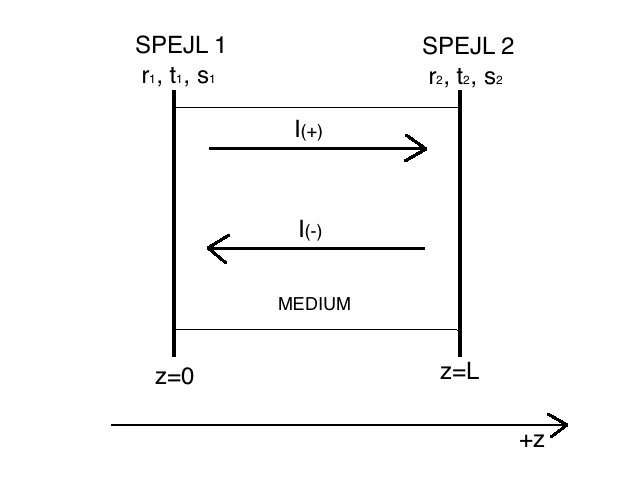
\includegraphics[width=0.7\textwidth]{Laserfysik/kavitet.png}
  \caption{Intensiteten af lys inde i en medium, der fylder hele kaviteten ud. $I^{(+)}$ betegner intensiteten, der rejser fra venstre mod højre, hvor $I^{(-)}$ betegner intensiteten, der rejser fra højre mod venstre.}
  \label{fig:kavitet}
\end{figure}

I grænserne $z=0$ og $z=L$ må der gælde for $I^{(+)}$ og $I^{(-)}$ at 
\begin{equation}
I^{(+)}(0) = r_1I^{(-)}(0) \,\,\,\,\, \text{og} \,\,\,\,\, I^{(-)}(L) = r_2I^{(+)}(L). 
\label{eq:graense1}
\end{equation}

Vi antager stadig, at intensiteten ikke ændrer sig i tid, hvorfor vi kan bruge ligning \ref{I_diff} og \ref{I_losning} til at beskrive $I^{(+)}$ og $I^{(-)}$. Vi får da 
\begin{equation}
\d{I^{(+)}}{z} = g(\nu)I^{(+)} \,\,\,\,\, \text{og} \,\,\,\,\, \d{I^{(-)}}{z} = -g(\nu)I^{(-)}
\label{eq:inten}
\end{equation}

med løsningerne 

\begin{equation}
I^{(+)}(z) = I^{(+)}(0)e^{g(\nu)z} \,\,\,\,\, \text{og} \,\,\,\,\,  I^{(-)}(z) = I^{(-)}(L)e^{g(\nu)(L-z)}.
\label{eq:intenlosning}
\end{equation}

I grænserne $z=L$ og $z=0$ er $I^{(+)}$ og $I^{(-)}$ hhv. 

\begin{equation}
I^{(+)}(L) = I^{(+)}(0)e^{g(\nu)L} \,\,\,\,\, \text{og} \,\,\,\,\, I^{(-)}(0) = I^{(-)}(L)e^{g(\nu)L}. 
\label{graenselosning}
\end{equation}

Kombineres ligningerne i \ref{eq:graense1} og \ref{graenselosning} fås (prøv selv at regne det ud)

\begin{equation}
I^{(+)}(0) = \left[ r_1r_2e^{2g(\nu)L}\right]I^{(+)}(0),
\end{equation}
som kun er opfyldt når 
\begin{equation}
r_1r_2e^{2g(\nu)L}=1. 
\end{equation}

Udnyttes regnereglen $\ln\left(e^x\right) = x$ fås tærskelværdien $g_t$ som

\begin{equation}
g_t \equiv g(\nu) = \frac{1}{2L}\ln\left(\frac{1}{r_1r_2}\right) = -\frac{1}{2L}\ln(r_1r_2). 
\label{eq:gt}
\end{equation}

Det er altså den værdi, som gevinst koeffcienten skal være større end eller lig med, for at forstærkningen af lyset inde i den optiske kavitet overgår tabene.

Såfremt spejlene har en meget høj reflektivitet, dvs. $r_1r_2>0,9$ kan ligning \ref{eq:gt} approksimeres til 

\begin{equation}
g_t = \frac{1}{2L}(1-r_1r_2).
\end{equation}

I dette tilfælde fylder mediet hele kaviteten, altså har kaviten en længde på $L$. Det er dog ikke en nødvendighed, og mediet kan altså godt kun fylde noget af kaviteten. Har mediet i stedet en længde $l$, som opfylder at $l<L$ er tærskelværdien 
\begin{equation}
g_t = \frac{1}{2l}(1-r_1r_2)
\end{equation}
i approksimationen for høj reflektivitet. 

\section{Rateligninger}
Inden for laserfysikken er man også interesseret i at kunne beskrive populationen i hver tilstand. I et 2--niveau system, som vi har arbejdet med indtil nu, ønsker vi at bestemmer, hvordan populationen $N_1$ og $N_2$ i tilstandene $1$ og $2$ ændrer sig i tid. Husk at $N_1$ og $N_2$ beskriver densiteter, dvs. $N_1 = n_1/V_m$ og $N_2 = n_2/V_m$, hvor $n_1$ og $n_2$ angiver antallet af atomer i hhv. tilstand 1 og 2, og $V_m$ angiver volumet af mediet, som de befinder sig i. 
Ligningerne, der beskriver ændringerne i populationerne kaldes \emph{rateligninger} og har et led, for hver proces, der bidrager til ændringer. 

\subsection{Spontan Emission}
Det første bidrag til rateligningerne i et 2--niveau system kommer fra spontan emission. Vi definerer raten for spontan emission, $A_{21}$, som raten hvormed $N_2$ i den høje energitilstand $E_2$ aftager, og $N_1$ i den lave energitilstand tilsvarende vokser. Vi kan altså beskrive ændringen i populationerne i forhold til spontan emission som 

\begin{equation}
\d{N_2}{t} = -A_{21}N_2 \,\,\,\,\, \text{og} \,\,\,\,\, \d{N_1}{t} = A_{21}N_2.
\label{eq:spontane}
\end{equation}

\subsection{Stimuleret Absorption og Emission}
Det andet bidrag kommer fra stimuleret absorption og emission. Det kan vises, at raten for ændringer i populationerne i forhold til stimuleret absorption er den samme som i forhold til stimuleret emission. Vi skal ikke vise det her, men det betyder, at raten hvormed antallet af atomer ændrer sig i tilstand 1 i forhold til stimuleret absorption er den samme som raten, hvormed antallet af atomer ændrer sig i tilstand 2 i forhold til stimuleret emission. I forhold til stimuleret absoprtion og emission har vi altså, at
\begin{align}
\d{N_2}{t} &= \text{(absorption rate)} \times N_1 - \text{(stimuleret emission rate)} \times N_2\\ &= \text{(absorption/emission rate)} \times (N_1-N_2)
\label{eq:stim1}
\end{align}
og 
\begin{equation}
\d{N_2}{t} = -\d{N_1}{t}. 
\label{eq:stim2}
\end{equation}

Raten for stimuleret emission må afhænge af antallet af indkommende fotoner, da de skal inducere processen. Tværsnittet, $\sigma(\nu)$, som tidligere beskrevet er det areal, som fotonerne skal befinde sig indenfor for at kunne inducere et atom til at undergå stimuleret emission. Kender vi antallet af indkommende fotoner pr. areal pr. tid, får vi antallet af fotoner pr. tid, hvilket vil svare til raten for stimuleret emission, altså
\begin{equation}
\text{stimuleret emission rate} = \sigma(\nu) \times \frac{\text{\# indkommende fotoner}}{\text{areal} \times \text{tid}}.
\end{equation}

\# indkommende fotoner kan udtrykkes ved intensiteten, i det 
\begin{equation}
I = \frac{\text{\# inkommende fotoner}}{\text{areal}\times \text{tid}}\cdot h\nu,
\label{eq:intensitetfoton}
\end{equation}
hvor $h\nu$ angiver energien af en enkelt foton. 

Absorption/emission raten bliver så 
\begin{equation}
\text{absorption/emission rate} = \sigma(\nu)\frac{I}{h\nu}.
\label{eq:rateea}
\end{equation}

Kombineres ligningerne \ref{eq:spontane}, \ref{eq:stim1}, \ref{eq:stim2} og \ref{eq:rateea} fås rateligningerne for populationerne i forhold til spontan emission, stimuleret absorption og stimuleret emission. 

\begin{align}
\d{N_2}{t} &= - \sigma(\nu)\frac{I}{h\nu}(N_2-N_1)-A_{21}N_2\\
\d{N_1}{t} &= \sigma(\nu)\frac{I}{h\nu}(N_2-N_1) + A_{21}N_2. 
\end{align}

\subsection{Kollisioner og Pumpning}
Det tredje bidrag kommer fra uelastiske kollisioner mellem atomerne. Et uelastisk stød giver anledning til en ændring i energien af atomer, hvorimod eleastiske stød ikke gør. Kollisionerne kan forårsage, at atomerne i tilstand 1 og 2 sparkes ud i uspecifiserede tilstande. Raterne hvormed dette sker skrives som hhv. $\Gamma_1$ og $\Gamma_2$. Kollisionerne vil give et negativt bidrag til rateligningerne, da de ''fjerner'' atomer. Rateligningerne bliver nu 
\begin{align}
\d{N_2}{t} &= -\Gamma_2 N_2- \sigma(\nu)\frac{I}{h\nu}(N_2-N_1)-A_{21}N_2\\
\d{N_1}{t} &= -\Gamma_1N_1 + \sigma(\nu)\frac{I}{h\nu}(N_2-N_1) + A_{21}N_2. 
\end{align}

Det fjerde og sidste bidrag kommer fra pumpningen. Pumpningen sørger for, at population inversionen $(N_2-N_1)$ er positiv, såldes at lasing opretholdes.  Raten for pumpningen skrives som $K$, det fås at

\begin{align}
\d{N_2}{t} &= -\Gamma_2 N_2- \sigma(\nu)\frac{I}{h\nu}(N_2-N_1)-A_{21}N_2 + K\\ &= -\left( \Gamma_2 + A_{21}\right)N_2 -g(\nu)\Phi+K\\
\d{N_1}{t} &= -\Gamma_1N_1 + \sigma(\nu)\frac{I}{h\nu}(N_2-N_1) + A_{21}N_2\\ &= -\Gamma_1N_1 + A_{21}N_2 + g(\nu)\Phi, 
\end{align}
hvor $\frac{I}{h\nu}$ beskriver \emph{fluxen}, der betegnes $\Phi$ og beskriver den totale intensitet pr. én fotons energi. 

\subsection{Rateligning for Fotonerne}
Udover at beskrive populationen af atomer i tilstand 1 og 2, er det også relevant at kunne beskrive populationen af fotoner i kaviteten. Til det skal vi igen se på intensiteten af lyset og bruge ligning \ref{eq:konti2}, der beskriver ændringen i intensiteten i forhold til tid og rum. Husk at sammenhængen mellem intensitet og antallet af fotoner er givet ved ligning \ref{eq:intensitetfoton}. Da vi nu ønsker at bestemme, hvordan antallet af fotoner ændrer sig i tid, kan vi ikke sætte $\d{I}{t}=0$ som gjort i ligning \ref{I_diff}. 

Situationen er den samme som givet på Figur \ref{fig:kavitet}, så $I^{(+)}$ og $I^{(-)}$ opfylder hhv. 
\begin{equation}
\d{I^{(+)}}{z} + \frac{1}{c} \d{I^{(+)}}{t} = g(\nu)I^{(+)} \,\,\,\,\, \text{og} \,\,\,\,\, -\d{I^{(-)}}{z} + \frac{1}{c} \d{I^{(-)}}{t} = g(\nu)I^{(-)}.
\end{equation}

Ligningerne lægges sammen, og det antages at variationen i $z$ mellem $I^{(+)}$ og $I^{(-)}$ er så lille, at leddet $I^{(+)}-I^{(-)}$ ikke bidrager. Vi antager altså, at rummet er uniformt, dvs. $\d{I}{z}=0$. Vi får så 
\begin{equation}
\d{}{t}\left[I^{(+)} + I^{(-)}\right] = cg(\nu)\left[I^{(+)}+I^{(-)}\right]. 
\label{eq:fotonrateeq}
\end{equation}

Da antallet af fotoner, $q$, er proportionalt med den totale intensitet kan vi omskrive ligning \ref{eq:fotonrateeq} til 
\begin{equation}
\d{q}{t} = cg(\nu)q,
\end{equation}
hvor $L$ er længden af kaviteten.

Antallet af fotoner vokser altså med raten 
\begin{equation}
cg(\nu),
\end{equation}
der kaldes \emph{vokseraten}. 

Men der går også noget lys/nogle fotoner tabt inde i kaviten bl.a. pga. spejlene, som tidligere nævnt. 
Raten for tabt intensitet findes ved at se på en rundtur i kaviteten for en enkelt foton (se Figur \ref{fig:intensitettab})

\begin{figure}[h!]
  \centering
  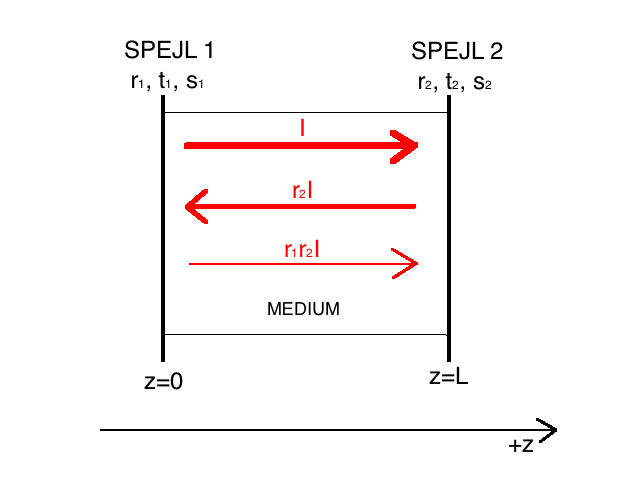
\includegraphics[width=0.7\textwidth]{Laserfysik/intensitettab.png}
  \caption{Intensiteten for én foton, der tager en tur rundt i kaviteten.}
  \label{fig:intensitettab}
\end{figure}

Der sker følgende:
\begin{itemize}
\item Fotonen rejser fra venstre mod højre med intensitet $I$. 
\item Fotonen rejser fra højre mod venstre med intensitet $r_2I$.
\item Fotonen rejser fra venstre mod højre med intensitet $r_1r_2I$.
\end{itemize}

En rundtur tager tiden $\frac{2L}{c}$ og ændringen i intensiteten er $I-r_1r_2I = (1-r_1r_2)I$, dvs. raten for tab i intensitet er 
\begin{equation}
\frac{c}{2L}(1-r_1r_2).
\end{equation}

Rateligningen for ændringen i population af fotoner er så 
\begin{equation}
\d{q}{t} = cg(\nu)q - \frac{c}{2L}(1-r_1r_2)q.
\end{equation}

\subsection{Omformulering af Rateligningerne}
Det er muligt at skrive rateligningerne for populationen af atomerne om, så de beskriver ændringen i antallet af atomer, $n_1$ og $n_2$, i stedet for densiterene, $N_1$ og $N_2$, som indtil nu. 
Til det behøves en omskrivning af $N_1$ og $N_2$, som er givet ved 
\begin{equation}
N_1 = \frac{n_1}{V_m} \,\,\,\,\, \text{og} \,\,\,\,\ N_2 = \frac{n_2}{V_m},
\end{equation}
som beskrevet tidligere, hvor $V_m$ er volumet af mediet, der i dette tilfælde udfylder hele kaviteten. 

Fluxen er samtidigt relateret til antallet af fotoner, $q$, ved 
\begin{equation}
\Phi = \frac{I}{h\nu} = \frac{cq}{V_m},
\end{equation}
og pumpningsraten $K$ er givet ved 
\begin{equation}
K = \frac{p}{V_m}.
\end{equation}

Dette giver rate ligningerne for $n_1$ og $n_2$
\begin{align}
\d{n_1}{t} &= -\Gamma_1n_1 + A_{21}n_2 + cg(\nu)q\\
\d{n_2}{t} &=-\left( \Gamma_2 + A_{21}\right)n_2 - cg(\nu)q + p.
\end{align}


\section{Flere--Niveau Laser Systemer}
Vi har indtil nu kun beskæftiget os med et 2--niveau system bestående af grundtilstanden(1) og en exciteret tilstand(2). Når et sådant system pumpes med stråling/fotoner vil de forårsage overgange mellem 1 og 2 pga. absorption og mellem 2 og 1 pga. stimuleret emission. 

Det bedste vi kan opnå i et 2--niveau system er at producere ca. lige mange atomer i hver tilstand, dvs. det ikke er muligt at opnå en positiv population inversion, hvor $N_2>N_1$. Det er derfor nødvendigt at indføre en tilstand mere og lave et 3--niveau system bestående af grundtilstanden og to exciterede tilstande(2 og 3) (se Figur \ref{fig:3niveau}). Stimuleret emission skal stadig foregå mellem tilstand 1 og 2, således at energien og bølgelængden af det ønskede laserlys ikke ændres. Tilstand 3 skal fungere som en \emph{pumpning tilstand}. Atomerne, der undergår absoprtion i tilstand 1 skal altså hoppe til tilstand 3 i stedet for tilstand 2. Dette kan opnåes ved at justere strålingen, som der pumpes med, så den har en energi, der svarer til energiforskellen mellem tilstand 1 og 3. 

\begin{figure}[h!]
  \centering
  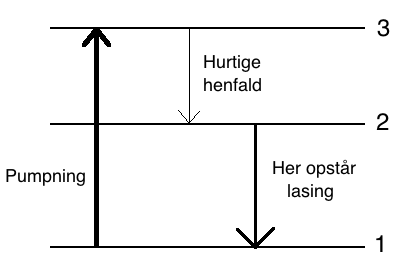
\includegraphics[width=0.5\textwidth]{Laserfysik/3niveau.png}
  \caption{3--niveau laser system.}
  \label{fig:3niveau}
\end{figure}

For at opnå en positiv population inversion må atomerne henfalde hurtigere fra tilstand 3 til 2 end de bliver pumpet fra tilstand 1 til 3. På den måde vil der hele tiden være flere atomer i tilstand 2 end tilstand 1. Henfaldene fra tilstand 3 til 2 kaldes derfor for \emph{hurtige henfald} og undergår typisk spontan emission eller kollisioner. Nogle atomer fra tilstand 3 kan i princippet også henfalde til tilstand 1, men det antages, at den mængde er væsentlig mindre end de, der henfalder til tilstand 2. 

Rateligningerne vil nu også ændre sig. Vi kalder nu $P$ for pumpe raten, hvor $PN_1$ vil være antallet af atomer/cm$^2$/s der er taget fra tilstand 1 til tilstand 3. Ændringen i populationen $N_1$ i forhold til pumpning er derfor 
\begin{equation}
\left( \d{N_1}{t}\right)_{p} = -N_1P.
\end{equation}

Da henfaldene fra tilstand 3 til 2 er hurtige, approksimeres det, at ændringen i populationen $N_2$ og $N_3$ i forhold til pumpning er ca. den samme, og må være den tilsvarende ændring, som populationen $N_1$ aftager med, altså 
\begin{equation}
\left(\d{N_2}{t}\right)_{p} \approx \left(\d{N_3}{t}\right)_{p} = -\left(\d{N_1}{t}\right)_{p} = PN_1.
\end{equation}

Udover stimuleret absorption og emission mellem tilstand 2 og 1 forekommer også spontan emission og kollisioner, der også skal tages højde for i rateligningerne, som tidligere beskrevet. Vi definerer nu en fælles rate for kollisioner og spontan emission fra tilstand 2 til 1, hvor det antages, at der ikke sker kollisioner eller spontan emission til andre uspecifiserede tilstande fra tilstand 2. Raten skrives derfor som $\Gamma_{21}$. Ændringen i $N_2$ i forhold til kollisioner og spontan emission må derfor være 
\begin{equation}
\left(\d{N_2}{t}\right)_{ke} = - \Gamma_{21}N_2,
\end{equation}
hvor $N_1$ må vokse med tilsvarende mængde, så 
\begin{equation}
\left(\d{N_1}{t}\right)_{ke} = \Gamma_{21}N_2
\end{equation}


Rateligningerne bliver nu 
\begin{align}
\d{N_1}{t} &= -N_1P + \Gamma_{21}N_2 + g(\nu)\Phi\\
\d{N_2}{t} &=N_1P - \Gamma_{21} - g(\nu)\Phi.
\end{align}

Som sagt antages det, at alle atomer i tilstand 3 henfalder til tilstand 2, dvs. $N_3=0$, og det giver derfor ikke nogen mening at opstille en rateligning for denne. \\

Et 3-niveau system kan optimeres yderligere ved at lave et 4-niveau system. 
Princippet er det samme, men nu er tilstand 1 ikke længere grundtilstanden, men en exciteret tilstand. Grundtilstanden kaldes nu for tilstand 0 (se Figur \ref{fig:4niveau}). 

\begin{figure}[h!]
  \centering
  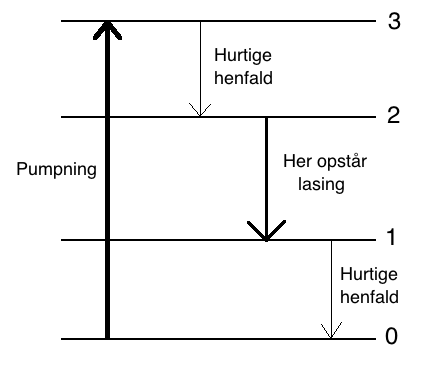
\includegraphics[width=0.5\textwidth]{Laserfysik/4niveau.png}
  \caption{4--niveau laser system.}
  \label{fig:4niveau}
\end{figure}

Pumpningen skal nu pumpe atomer fra tilstand 0 til tilstand 3, og hurtige henfald skal ske både fra tilstand 3 til 2 som i 3--niveau systemet, men også fra tilstand 1 til 0. De hurtige henfald skal stadig ske hurtigere, end der bliver pumpet. Ved at tilføje tilstand 0, kan tilstand 1 ''tømmes'', dvs. $N_1$ vil aftage. En aftagende $N_1$ vil resultere i en voksende positiv population inversion, $N_2-N_1$, hvilket er ønsket. 

Vi definerer nu raten, hvormed atomer henfalder fra tilstand 1 til 0 ved spontan emission og kollisioner som $\Gamma_{10}$. Rateligningerne for et 4--niveau system er så 

\begin{align}
\d{N_0}{t} &= -PN_0 + \Gamma_{10}N_1\\
\d{N_1}{t} &= -\Gamma_{10}N_1+\Gamma_{21}N_2 + g(\nu)\Phi\\
\d{N_2}{t} &= PN_0 - \Gamma_{21}N_2 - g(\nu)\Phi.
\end{align}


\section{Pulserende Laser med Q-switching}
Vi har indtil nu kun beskæftiget os med en \emph{kontinuert} laser, en såkaldt cw-laser, hvor cw står for \emph{continous wave}. 
En laser kan også være pulserende, dvs. lyset kommer ud i pulser i stedet for ud i et konstant flow. 

En metode til at lave en pulserende laser er \emph{Q-switching}, som vi lader beholde sit engelske navn. Q refererer til kvaliteten af kaviteten, hvor en høj Q vil svare til en kavitet med lave tab, og omvendt for en lav Q. 

Princippet er, at man starter med en kavitet, der har en lav Q, dvs. kaviteten har store tab, og det er derfor ikke muligt at opnå lasing. Pumpes mediet inde i kaviteten pludseligt meget hårdt, vil det resultere i en pludselig høj rate for stimuleret emission, og der vil ske en hurtig udsendelse af lys. Resultatet er altså en kort, intens laserpuls, der typisk varer mellem $10^{-8}$--$10^{-7}$s. I nogle af laserlaboratorierne er pulserne endnu kortere, og kan vare helt ned til picosekunder, dvs. $10^{-12}$ s, disse kan dog ikke opnåes med Q-switching men med en metode, der hedder \emph{mode locking}, som vi ikke skal berøre yderligere. Det er hurtigere end noget elektronisk udstyr kan nå at måle, og man måler derfor varigheden af så korte pulser ved at manipulere lyset med optiske elementer. 

En Q-switched pulserende laser kan opnåes med forskellige metoder for Q-switching. Den første metode er et \emph{roterende spejl} (se Figur \ref{fig:rotspejl}). 
Mediet ligger inde i kaviteten, der består af to spejle, hvoraf en af dem er roterende. Når det roterende spejl ikke står parallelt med det andet, vil kaviten have en meget lav Q. Prøv selv, at indse hvorfor. Når spejlene derimod står helt parallelt, vil der opstå en pludselig høj rate for stimuleret emission, og en laserpuls udsendes. 

\begin{figure}[h!]
  \centering
  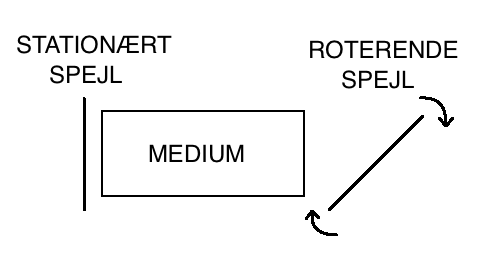
\includegraphics[width=0.5\textwidth]{Laserfysik/rotspejl.png}
  \caption{Q--switching med roterende spejl.}
  \label{fig:rotspejl}
\end{figure}

Den anden metode er at benytte en mættelig absorber. Et sådan element bruges som et medium og indsættes i en optisk kavitet, hvorefter det pumpes. I det første stykke tid absorberer mediet så meget af lyset, at kaviteten har store tab og derfor en lav Q. Men på et tidspunkt kan det ikke absorbere mere lys, og mediet siges at være \emph{mættet}. Mediet bliver nu transparent for lyset inde i kaviteten, der får en høj Q, og derved udsender en laserpuls. 

Den tredje og sidste metode kræver forståelse for polariseret lys, som vil blive gennemgået i detalje i valgemnet om Elektromagnetiske Bølger. Kort fortalt er polariseret lys, noget lys, hvis elektriske felt bevæger sig i en bestemt retning. Denne retning kan manipuleres ved at sende lyset gennem bestemte optiske elementer. I dette eksempel benyttes \emph{lineært polariseret} lys og \emph{cirkulært polariseret} lys. Hvis lyset er linært polariseret betyder det, at det elektriske felt af lyset bevæger sig lineært, f.eks. horisontalt eller vertikalt. Hvis lyset er cirkulært polariseret, betyder det, at det elektriske felt bevæger sig i cirkler, enten til højre eller venstre. 
Metoden bruger en elektrisk-optisk enhed, der er påvirket af en elektrisk spænding. Denne samt en \emph{lineær polarisator} er placeret i en optisk kavitet sammen med mediet (se Figur \ref{fig:elektriskoptisk}). En lineær polarisator tillader kun lineært polariseret lys i en bestemt retning at komme igennem. Det antages, at denne lineære polarisator kun tillader at lade vertikalt lys komme igennem. 

\begin{figure}[h!]
  \centering
  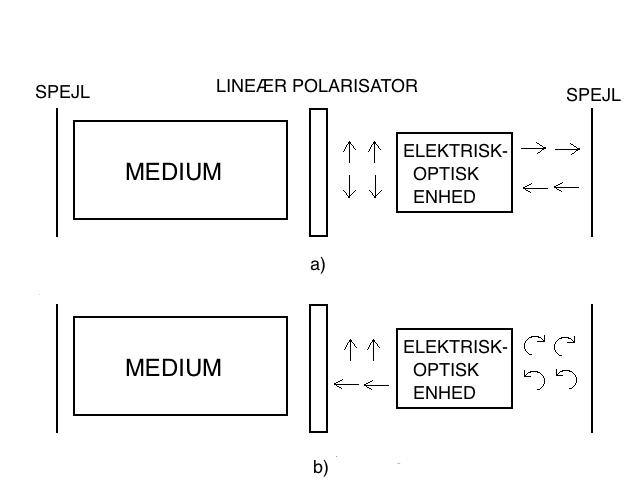
\includegraphics[width=0.7\textwidth]{Laserfysik/elektriskoptisk.png}
  \caption{Q--switching med elektrisk--optisk enhed. a) Elektrisk--optisk enhed fungerer som halvbølge plade, så lasing er opnået. b) Elektrisk--optisk enhed fungerer som kvartbølge plade, så lasing er ikke opnået.}
  \label{fig:elektriskoptisk}
\end{figure}

Den elektrisk-optiske enhed kan enten fungere som en \emph{halvbølge plade} eller en \emph{kvartbølge plade} afhængig af den pålagte spænding. En halvbølge plade kan rotere lysets polarisation med en vinkel, hvor en kvartbølge plade kan gøre lineært polariseret lys til cirkulært polariseret lys og omvendt. 
Når den elektrisk-optiske enhed fungerer som en halvbølge plade i denne opstilling roteres lyset med $90\degree$, dvs. vertikalt polariseret lys bliver til horisontalt polariseret lys og omvendt. Bemærk, at en halvbølge plade ikke altid roterer lyset med $90\degree$, men at det kræver en specifik indstilling af halvbølgepladen. 

Figur \ref{fig:elektriskoptisk} viser opstillingen. Når lyset generes i mediet, rejser det fra venstre mod højre ind gennem den lineære polaristor, hvor kun vertikalt polariseret lys kan komme igennem. Hvis den elektrisk-optiske enhed fungerer som en halvbølge plade vil lyset blive horisontalt polariset inden det rammer spejlet. Det horisontale polariserede lys reflekteres i spejlet og går tilbage ind i den elekrisk-optiske enhed, hvor lyset igen bliver roteret $90\degree$, dvs. lyset nu er vertikalt polariseret igen og kan fortsætte gennem den lineære polarisator, hvorefter det går tilbage ind i mediet og bidrager til forstærkningen af lyset. Der sker en pludselig høj rate for stimuleret emission, som giver anledning til en laserpuls. 
Hvis den elektrisk-optiske enhed i stedet fungerer som en kvartbølge plade, vil det vertikalt polariseret lys blive cirkulært polariseret inden det rammer spejlet. Lad os sige, det cirkulerer til højre. Når højre cirkulært polariseret lys reflekteres i spejlet, vil lyset skifte retning, dvs. lyset nu vil cirkulere til venstre, inden det går tilbage ind i den elektrisk-optiske enhed. Hvis vertikalt polariseret lys bliver til højre cirkulært polariset lys efter enheden, så må venstre cirkulært polariseret lys blive til lineært horisontalt polariseret lys efter enheden, når det rejser tilbage. Det horisontale polariserede lys kan \emph{ikke} gå igennem den lineære polaristor, og der vil derfor ikke komme lys tilbage i mediet. Lyset vil ikke forstærkes og lasing er ikke opnået. 

Om den elektrisk-optiske enhed fungerer som en halvbølge plade eller kvartbølge plade afhænger af den spænding, som enheden påvirkes med. Ved at variere spændingen, således at enheden står og veksler mellem at være det ene eller andet, vil et tog af laserpulser opstå, når den virker som en halvbølge plade. 


